\chapter{D'Alembert Principle and Lagrange's Equations}
In classical mechanic problems were described by Newtons 3N\footnote{Each of
the N particles has three degrees in a three dimensional space.} differential
equations\footnote{Also called equations of motion.} of 2nd order 
\begin{equation}
  m_i \ddot{\vec r_i} \,=\, \vec F_i^{(e)} \sum_{i \neq j} \vec F_{ij},
\end{equation}
where $\vec F^{(e)}$ denotes the external force and $F_{ij}$ the internal forces
acting on the system. As many systems contain a lot of particles the Newton
approach gets very unhandy, leading to the easier to handle \textit{D'Alembert's
principle} and \textit{Lagrange equations}. First step to develop these new
technics is to introduce \textit{constraints}. 

\section{Constraints}
Many systems underly forces of constraints, which can be denoted as 
\begin{equation}
  \label{holonomicConstraint}
  f(\vec r_1, \vec r_2, \cdots, \vec r_N, t) \,=\, 0.
\end{equation}
Every force of constraints reduces the degress of freedom. A system of N
particles has 3N degrees of freedom a system including p forces of
constraints then has only
\begin{equation}
  S \,=\, 3N - p
\end{equation}
degrees of freedom left. 

Until now we considered working in the classical way with \textit{cartesian
coordinates}. Due to the forces of constraints some of the cartesian coordinates $\vec
r_i$ are now linearly dependent, hence the \textit{equations of motion} are not
all independent. To get the full advantage of using constraints we have to
introduce \textit{generalized coordinates}. Meaning that we can choose S
totally arbitraily coordinates, which just have to be linearly
independent to describe our N particle system completly. 

The only problem that is left is, that \textit{forces of constraints} are
unkown a priori. Consequently we should like to formulate our theory in a way,
that the \textit{forces of constraints} disappear automatically, which will be 
done with \textit{D'Alembert's principle}. 

\section{D'Alembert's principle}
To derive \textit{D'Alembert's principle} we have to introduce the virtual
displacements $delta \vec r$. Virtual displacements is an \textbf{assumed}
infinitesimal change of system coordinates occuring while \textbf{time is held
constant}\footnote{Virtual displacements cannot take part in our real world
because time is held constant, there is no movement without time. That's why
the displacement is called virtual.}. Apart from that virtual displacement are
mathematically treated as a normal displacement $d \vec r$. 

Regarding a system equilibrium, we know that the \textit{total
force}\footnote{External and internal force on a particle.} on each particle
vanishes $\vec F_i \,=\, 0$. Furthermore the classical work is given by $dW
\,=\, \vec F \cdot d \vec r$, thus we can define the virtual work as
\begin{equation}
  \delta W \,=\, \vec F \cdot \delta \vec r.
\end{equation}
Consequently, due to the vanishing total force, the sum over the total virtual
work must also vanish
\begin{equation}
  \label{netVirtualWork}
  \sum_{i} \vec F_i \cdot \delta \vec r \,=\, 0.
\end{equation}
To obtain \textit{D'Alemberts principle} we can now split up the total force
$\vec F_i$ into so called \textit{applied forces} $F^{(a)}$ \footnote{Simply all forces, but the
forces of constraint.} and the \textit{forces of constraint} $f$
\begin{equation}
  \vec F \,=\, \vec F^{(a)} + \vec f \quad \Rightarrow \quad \vec F^{(a)} +
\vec f - \vec F \,=\, 0 
\end{equation}
Thus we can write for the net virtual work eq.~(\ref{netVirtualWork})
\begin{equation}
  \sum_{i} (\vec F_i^{(a)} - \vec F_i) \cdot \delta \vec r + \sum_{i} \vec f_i \cdot \delta \vec r
\,=\, 0
\end{equation}
Now we seperated the \textit{forces of constraints} from the applied forces and
physical evidence shows that
\begin{equation}
  \sum_{i} \vec f \cdot \delta \vec r \,=\, 0.
\end{equation}
We cannot prove this fact, but merely have to accept it!\footnote{Goldstein
restricts himself for systems with a vanishing net virtual work of the forces
of constraints. Excluding all other cases or a derivation.} Hence we are left
with
\begin{equation}
  \label{dAlembertPrinciple}
  \sum_{i} (\vec F_i^{(a)} - \dot{\vec p_i}) \cdot \delta \vec r \,=\, 0 \quad
\text{with} \quad \vec F \,=\, m \ddot{\vec r} \,=\, \dot{\vec p},
\end{equation}
which is referred to as \textit{D'Alembert's princple}.

Having achieved our aim to cause to vanish the forces of constraints we still
are left with linearly dependent virtual displacements $\delta \vec
r$\footnote{The cartesian coordinates $\vec r$ have been linearly dependent,
due to the forces of constraint, and so are $\delta \vec r$.}. As before we
want to replace those by independent generalized coordinates $q_i$.

Droppign the superscript of $\vec F_i^{(a)} \,\to\, \vec F_i$ in
eq.~(\ref{dAlembertPrinciple}) we now want to evaluate the terms $\vec F_i
\cdot \delta \vec r$ and $- \dot{\vec p_i} \cdot \delta \vec r$ yielding the
\textit{d'Alembert principle} in form of the generalized coordinates $\vec
q_i$. Starting with the first one we need to make use of the total derivative
of the virtual displacement $\delta \vec r$\footnote{$\delta \vec r$ is only
dependent on the generalized coordinates $\vec q_i$ and not on the time t.}
given by
\begin{equation}
  \delta \vec r_i \,=\, \sum_j \frac{\partial \vec r_i}{\partial q_j} \delta
q_i 
\end{equation}
Hence for $\sum_i \delta F_i \cdot \delta \vec r$ we get
\begin{equation}
  \label{dAlembertFirst}
  \begin{aligned}
    \sum_i \vec F_i \cdot \delta \vec r \,=\,& \sum_i \sum_j \vec F_i \cdot
\frac{\partial \vec r_i}{\partial q_j} \delta q_j \\
    \,=\,& \sum_i Q_j \delta q_j,
  \end{aligned}
\end{equation}
where we defined the \textit{generalized force} $Q_j$ 
\begin{equation}
  \label{generalizedForce}
  \vec Q_j \,=\, \sum_i \vec F_i \frac{\partial \vec r_i}{\partial q_j}.
\end{equation}
Before evaluating the second term, we need to introduce to
idendities, which we are not going to derive here\footnote{We already derived these in our first exercise sheet.} :
\begin{align}
  \frac{\vec r_i}{q_j} \,=\,& \frac{\dot{\vec r}}{\dot{q_j}} \\
  \frac{d}{dt} \frac{\vec r_i}{q_j} \,=\,& \frac{\dot{\vec r_i}}{q_j}
\end{align}
With these two identities we are able to evaluate the second expression
\begin{equation}
  \label{dAlembertSecond}
  \begin{aligned}
    \sum_i \dot{\vec p_i} \cdot \delta \vec r \,=\,& \sum_i \sum_j m_i \ddot{\vec
r_i} \cdot \frac{\partial \vec r_i}{\partial q_j} \delta q_j \\
    \,=\,& \sum_i \sum_j m_i \left[\frac{d}{dt}\left(\dot{\vec r_i}  \frac{\partial \vec r_i}{\partial
q_j}\right) - \dot{\vec r_i} \frac{d}{dt} \frac{\partial \vec r_i}{\partial q_j} \right] \delta q_j
\\
    \,=\,& \sum_i \sum_j m_i \left[\frac{d}{dt} \left(\dot{\vec r_i} \frac{\partial
\dot{\vec r_i}}{\dot{q_j}}\right) - \dot{\vec r_i} \frac{\dot{\partial \vec
r_i}}{\partial q_j}\right] \delta q_j \\
    \,=\,& \sum_i \sum_j m_i \left\{\frac{d}{dt} \left[ \frac{\partial}{\partial
\dot q_j}\left(\frac{1}{2} \dot{\vec r_i^2}\right)\right] - \frac{\partial}{\partial
q_j} \left(\frac{1}{2} \dot{\vec r_i^2} \right)\right\} \delta q_j \\
    \,=\,& \sum_j \left\{ \frac{d}{dt} \left(\frac{\partial T}{\partial \dot
q_j}\right) - \frac{\partial T}{\partial q_j} \right\} 
  \end{aligned}
\end{equation}
Plugging now our first term eq.~(\ref{dAlembertFirst}) and our second term
eq.~(\ref{dAlembertSecond}) in \textit{d'Alembert's principle}
eq.~(\ref{dAlembertPrinciple}) yields 
\begin{equation}
  \label{dAlembertPrinciple2}
  \sum_j \left\{ \left[\frac{d}{dt} \frac{\partial T}{\partial \dot q_j} -
\frac{\partial T}{\partial q_j}\right] - Q_j \right\} \delta q_j \,=\, 0
\end{equation}
From this point we will derive within a few steps the desired
\textit{Lagrange's equations}.

\section{Lagrange's equations}
To finally get \textit{Lagrange's equations} we need to regard a
\textit{conservative system} with \textit{holonomic
constraints}\footnote{Constraints of the form defined in
eq.~(\ref{holonomicConstraint}).}. 

\textit{Holonomic constraints} lead to independent \textit{generalized
coordinates} $q_j$. Thus we can choose $\delta q_j$ arbitrarily, so that not
the sum, but every single coefficient has to be zero. Hence the sum from
\textit{d'Alembert's principle} eq.~(\ref{dAlembertPrinciple2}) vanishes
\begin{equation}
  \left\{ \left[\frac{d}{dt} \left(\frac{\partial T}{\partial \dot q_j} \right) -
\frac{\partial T}{q_j} \right]- Q_j \right\} \delta q_j \,=\, 0
\end{equation}

For a \textit{conservative system} we can define a potential $V(\vec r_1, \vec
r_2, \cdots, \vec r_N)$ depending only on radi vectors (not on velocities
$\dot{\vec r_i}$), which is responsible for our \textit{applied force}
\begin{equation}
  \vec F_i^{(a)} \,=\, -\nabla_i V.
\end{equation}
Consequently we can write for our \textit{generalized Force}
eq.~(\ref{generalizedForce}) 
\begin{equation}
  Q_j \,=\, \sum_i \vec F_i \frac{\partial \vec r_i}{\partial q_j} \,=\,
- \sum_i \nabla_i V \frac{\partial \vec r_i}{\partial q_j} \,=\,
-\frac{V}{q_j}, 
\end{equation}
because $\nabla_i \cdot \partial \vec r_i$ cancel out.

Thus for a \textit{conservative system} with \textit{holonomic constraints} we
get
\begin{equation}
  \left\{ \frac{d}{dt} \left[\frac{\partial T}{\partial \dot q_j} - \frac{\partial
T}{\partial q_j} \right] + \frac{V}{q_j}\right\} \delta q_j \,=\, \left[
\frac{d}{dt} \frac{\partial T}{\dot q_j} - \frac{\partial (T - V)}{\partial
q_j} \right] \delta q_j 
\end{equation}
Now we can define the \textit{Lagrange function}
\begin{equation}
  L(q_1, \cdots q_N, \dot q_1, \cdots \dot q_N, t) = T(q_1, \cdots, q_N, \dot
q_1, \cdots \dot q_N, t) - V(q_1, \cdots, q_N).
\end{equation}
Due to the fact, that $V(q_1, \cdots, q_N)$ does not depend on the velocities $\dot
q_i$ we can include $V$ in the partial derivative with respect to $\cdot q_j$
\begin{equation}
\left[ \frac{d}{dt} \frac{\partial (T-V)}{\dot q_j} - \frac{\partial (T - V)}{\partial
q_j} \right] \delta q_j  \,=\, \left[ \frac{d}{dt} \frac{\partial L}{\dot q_j}
- \frac{\partial L}{\partial
q_j} \right] \delta q_j
\end{equation}
The above equations are reffered to as \textit{Lagrange's equations}.

We now obtained a mechanism using energy and work (T - V) instead of momentum
and force, as we have been used from the newton mechanic. We now have to deal
with S differential equations of 2nd order. Consequently 2S initial editions
are needed to solve for the \textit{equations of motions}.

\section{Exercise}

\subsection{Task}
\begin{figure}[h]
    \centering
    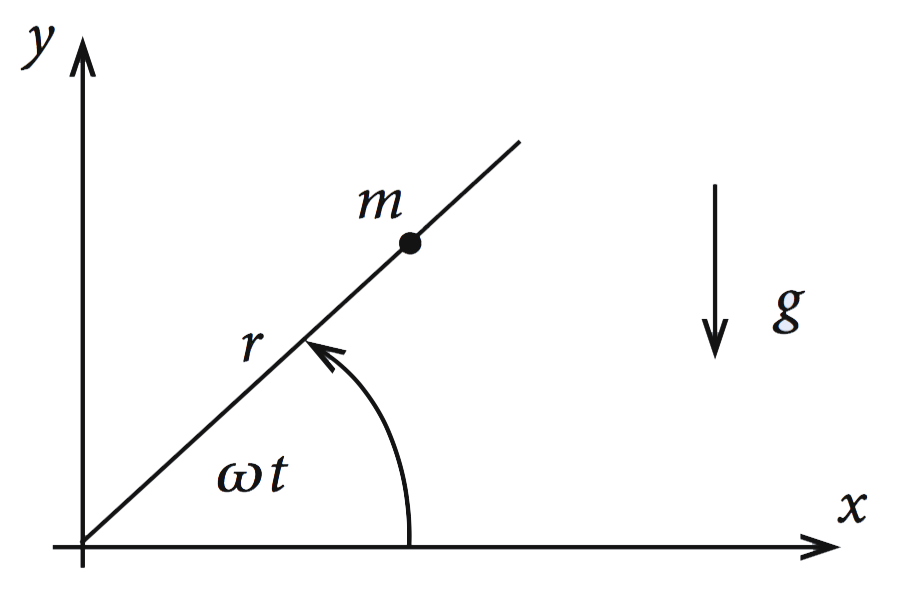
\includegraphics[width=0.5\textwidth]{images/exercises_1_1.png}
    \caption{Awesome Image}
    \label{fig:awesome_image}
\end{figure}
Regard a particle with mass $m$ moving without friction on a wire, which rotates with a
constant velocity $\omega$ around its origin. The movement of the particle is
influenced by the gravitation $g$.
\begin{enumerate}
  \item Formulate the constraints.
  \item Define the Lagrangian of the particle.
  \item Solve for Lagrange's equations and find the general solution for r(t).
motion 
  \item Use the initial conditions
    \begin{equation*}
      r(t=0) \,=\, r_0 \quad \text{and} \dot r(t=0) \,=\, 0
    \end{equation*}
    to get the equations of motion.
  \item Solve the problem with classical Newton mechanics.
\end{enumerate}

\subsection{Solution}
\subsubsection{1.} 
The constraints are given by
\begin{align*}
  z \,=\,& 0 \\
  y - x \tan(\omega t) \,=\, 0
\end{align*}
Consequently we can reduce the degrees of freedom from 
\begin{equation*}
  S \,=\, 3 - 2 \,=\, 1
\end{equation*}
An apropriate generalized coordinate would be $q(t) \,=\, r(t)$.
\subsubsection{2.}
To find the Lagrangian we first need a relation between the cartesian
coordinates and their polar corespondent
\begin{alignat*}{2}
 x \,=\,& r \cos(\omega t)  &\quad y \,=\,& r \sin(\omega t) \\   
 \dot x \,=\,& -\dot r \cos(\omega t) + r \omega \sin(\omega t)   & \dot y  
    \,=\,& \dot y \sin(\omega t) + r \omega \cos(\omega t) 
\end{alignat*}
Then we need to find the kinetical energy
\begin{equation*}
  T \,=\, \frac{1}{2} m \vec v^2 \,=\, \frac{1}{2} m ( \dot x^2 + \dot y^2 )
\,=\, \frac{1}{2} m ( \dot r^2 + r^2 \omega^2 )
\end{equation*}
The potential energy is then obviously given by
\begin{equation*}
  V \,=\, mgh \,=\, mg r \sin(\omega t)
\end{equation*}
Hence for the Lagrangian
\begin{equation*}
  L \,=\, T - V \,=\, \frac{1}{2} m (\dot r^2 + r^2 \omega^2) - mg r \sin
(\omega t)
\end{equation*}
\subsubsection{3.}
The Lagrange equation is given by
\begin{equation*}
  \frac{d}{dt} \frac{\partial L}{\partial \dot r} - \frac{\partial L}{\partial
r} \,=\, 0.
\end{equation*}
Hence
\begin{equation*}
  \frac{d}{dt} \frac{\partial L}{\partial \dot r} \,=\, m \ddot r \quad
\text{and} \quad \frac{\partial L}{\partial r} \,=\, mr\omega^2 - mg
\sin(\omega t).
\end{equation*}
Combined we get the following differential equation
\begin{equation*}
   \ddot r - r \omega^2 + g\sin(\omega t) \,=\, 0.
\end{equation*}
To find the general solution we start with the homogenous equation 
\begin{equation*}
  \ddot r - r\omega^2 \,=\, 0.
\end{equation*}
Which can be solved with the ansatz
\begin{equation*}
  r_0(t) \,=\, \alpha e^{\omega t} + \beta e^{-\omega t}.
\end{equation*}
To get the general solution we now have to find a special solution and add it
to the homogeneous solution. The following ansatz will serve us well
\begin{equation*}
  r_s(t) \,=\, \gamma \sin(\omega t) \quad \Rightarrow \quad \ddot r_s(t) \,=\,
-\gamma \omega^2 \sin(\omega t).
\end{equation*}
Plugging the above relations into our Lagrange equation yields
\begin{equation*}
  - \gamma \omega^2 \sin(\omega t) - \gamma \omega^2 \sin(\omega t) + g
\sin(\omega t) \,=\, 0 \quad \Rightarrow \quad \gamma \,=\, \frac{g}{2\omega^2}  
\end{equation*}
And thus for our general solution (adding homogeneous and special solution) 
\begin{equation*}
  r(t) \,=\, \alpha e^{\omega t} + \beta e^{-\omega t} + \frac{g}{2\omega^2}
\sin(\omega t)
\end{equation*}
\subsubsection{4.}
Pluggin the initial conditions
\begin{equation*}
  r(0) \,=\, r_0 \quad \text{and} \quad \dot r(0) \,=\, 0 
\end{equation*}
into our general solution
\begin{align*}
  r(t) \,=\,& \alpha e^{\omega t} + \beta e^{-\omega t} + \frac{g}{2\omega^2}
\sin(\omega t) \\
  \dot r(t) \,=\,& \alpha \omega e^{\omega t} - \beta \omega e^{-\omega t} +
\frac{g}{2\omega} \cos{\omega t}
\end{align*}
yields
\begin{align*}
  \alpha + \beta \,=\,& r_0 \\
  \alpha - \beta + \frac{g}{2\omega} \,=\,& 0 \quad \Rightarrow \quad \alpha
\,=\, \beta - \frac{g}{2\omega^2}
\end{align*}
Hence plugin the $\alpha$ from the second line into the first yields
\begin{equation*}
  2\beta - \frac{g}{2\omega^2} \,=\, r_0 \quad \Rightarrow \quad \beta \,=\,
\frac{r_0}{2} + \frac{g}{4\omega^2}
\end{equation*}
and 
\begin{equation*}
  \alpha \,=\, \frac{r_0}{2} - \frac{g}{4\omega^2}.
\end{equation*}
Pluggin $\alpha$ and $\beta$ in our general solution we get
\begin{equation*}
  r(t) \,=\, \frac{r_0}{2} \left(e^{\omega t} + e^{-\omega t}\right) -
\frac{g}{4\omega^2} \left(e^{\omega t} - e^{-\omega t}\right) +
\frac{g}{2\omega^2} \sin(\omega t)
\end{equation*}
\subsubsection{5.}
To solve the system in the Newtonian way we first need to formulate the forces
of constraints, which is not that simple. Anyway we are left with the
gravitational force $\vec F_g$ and the zentrifugal force $\vec F_z$
\begin{equation*}
  m \ddot r \,=\, \vec -F_g + \vec F_z.
\end{equation*}
The gravitational force is simply given by
\begin{equation*}
  \vec F_g \,=\, m g \sin(\omega t) 
\end{equation*}
whereas the zentrifugal force is defined as
\begin{equation*}
  \vec F_z \,=\, - m ( \vec \omega \times ( \vec \omega \times \vec r ) ) \,=\, -
m( \vec \omega (\vec \omega \cdot \vec r) - \vec r (\vec \omega \cdot \vec
\omega)) \,=\, m r \omega^2 
\end{equation*}
where we used the triple cross product identity $\vec a \times ( \vec b \times
\vec c) \,=\, \vec b (\vec a \cdot \vec c) - \vec c( \vec a \cdot b )$, and the
fact that $\vec \omega$ is orthogonal to $\vec r$. Hence 
\begin{equation*}
  m \ddot r - m r \omega^2 + m g\sin(\omega t) \,=\, 0,
\end{equation*}
which is exactly the same as our Lagrangian equation in the 3rd part.
